\documentclass[12pt]{article} 
\usepackage[brazil]{babel} %hifenização em português do brasil
\usepackage{gensymb}
\usepackage[pdftex]{hyperref}
\usepackage[T1]{fontenc} % caracteres com acentos são considerados um bloco só
\usepackage{graphicx}
\usepackage{ae} %arruma a fonte quando usa o pacote acima
\usepackage[utf8]{inputenc}
\usepackage{graphicx}%Para inserir figuras

\usepackage{cite}

\begin{document} % Aqui começa o documento
\title{Implementação \textit{system calls} no kernel linux V. 4.13.12\vspace{3.5cm}} % título

\author{
	João Paulo de Oliveira
	\texttt{joaopaulodeoliveira123@gmail.com}
	\and
	Lucas Rossi Rabelo
	\texttt{lucasrossi98@hotmail.com}
	\and		
	Matheus Pimenta Reis
	\texttt{}
	\vspace*{9cm}
}

\maketitle
\tableofcontents

\pagebreak
\section*{Implementação \textbf{System Calls} no Linux}
As \textit{System Calls} fazer o interfaceamento entre o hardware e os processo do espaço de usuário, elas também servem para três propósitos principais:
\begin{enumerate}
	\item Provém abstração com o hardware para que o usuário tenha um maior rendimento. Por exemplo, o usuário não se preocupa com o tipo de partição em que ele lerá um arquivo;
	\item As \textit{system calls} garantem a segurança e estabilidade para que um usuário relativamente leigo possa ter um alto rendimento com gerência de permissão, usuários e outros critérios de gerência do kernel;
	\item Uma camada entre espaço de usuário e o resto do sistema permite fornece o sistema virtualizado para os processos.
\end{enumerate}
	As chamadas syscalls em linux são, na maioria dos casos, acessadas pelas funções definidas na C library. As syscalls em si retornam um valor do tipo long4 que, quando negativo, em geral, denota um erro, já o retorno com valor zero (nem sempre) é um sinal de sucesso. A C library, quando uma \textit{system call} retorna um erro, ela grava o código desse erro na variável global errno, que pode ser ser traduzida para um texto que fala sobre o erro através de funções de biblioteca.
	
	Para a implementação de uma \textit{system call} deve-se ter acesso ao código do kernel do sistema operacional para tanto, foi escolhido o kernel Linux que é open source.
\subsection*{Download do Kernel}
Por ser open source, o código fonte do kernel do Linux é mantido online para livre acesso no GitHub(\url{https://github.com/torvalds/linux}), e também em The Linux Kernel Archives (\url{https://www.kernel.org/}) em várias versões e formatos de arquivos(compactados). A versão mais recente dado a data de início do TCD foi a versão \textbf{14.13.12}.
de gerência do kernel.
	A Free Software Foundation mantém, gerencia e presta suporte para o The Linux Kernel Archives.O donwnload do kernel pode ser feito facilmente, além de outras funções com perguntas frequentes, download de versões em teste (beta) para ser compilado em qualquer distribuição linux ou em outras plataformas que suportam o kernel.
	\vspace*{2cm}
	 Como pode ser visto na imagem abaixo:
\begin{figure}[!h]
	\centering
	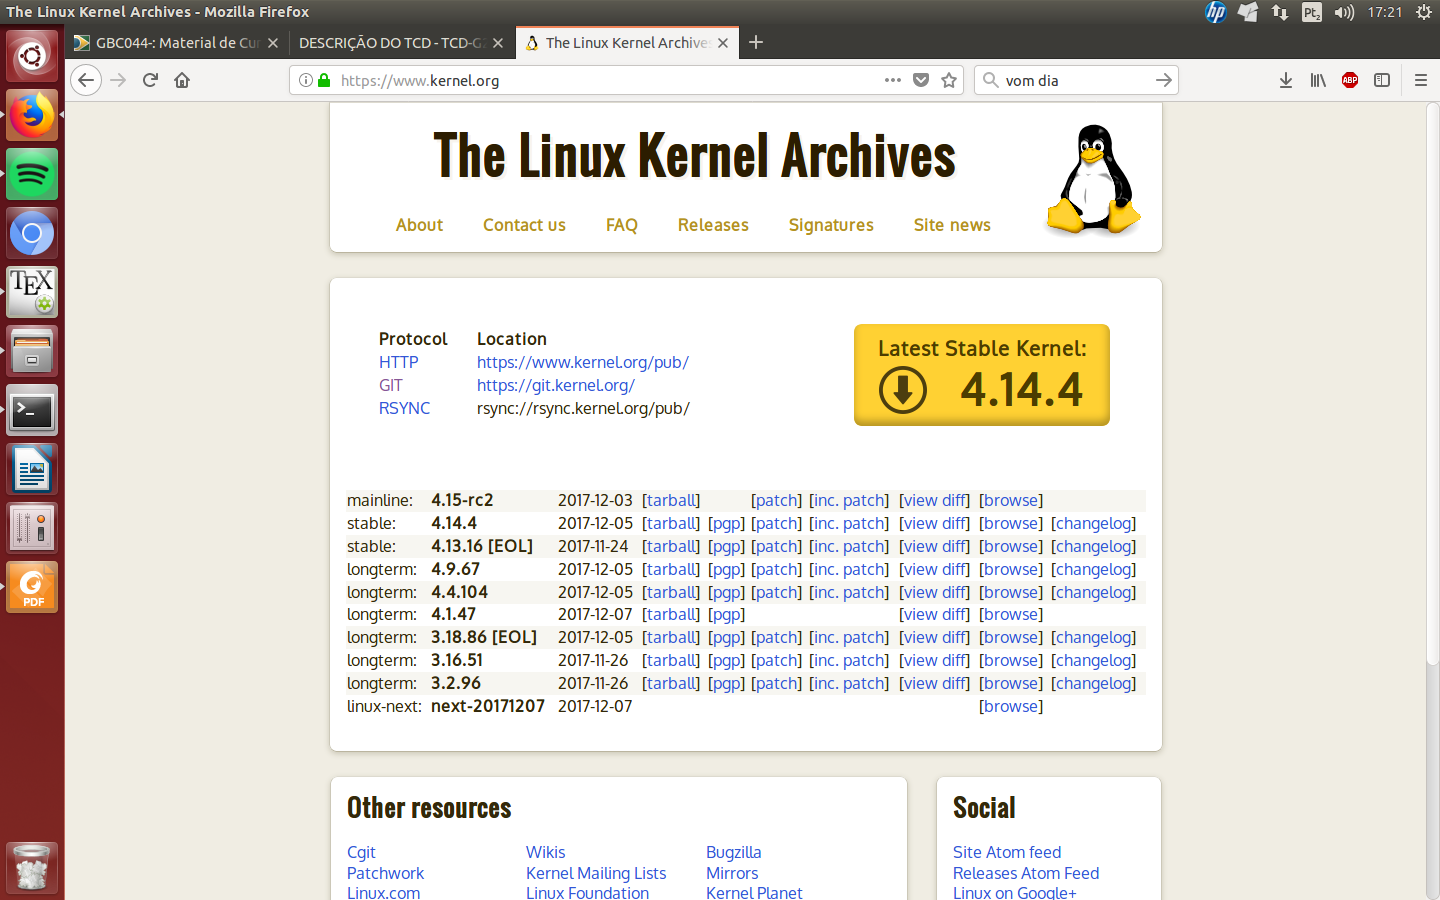
\includegraphics[scale=0.2]{imagens/kernelorg.png}
	\caption{The Linux Kernel Archives: Local de download do Kernel}
	\label{kernelorg}
\end{figure}

\subsection*{Download do Kernel}
Por ser open source, o código fonte do kernel do Linux é mantido online para livre acesso no GitHub(\url{https://github.com/torvalds/linux}), e também em The Linux Kernel Archives (\url{https://www.kernel.org/}) em várias versões e formatos de arquivos(compactados). A versão mais recente dado a data de início do TCD foi a versão \textbf{14.13.12}.
de gerência do kernel.
	A Free Software Foundation mantém, gerencia e presta suporte para o The Linux Kernel Archives.O donwnload do kernel pode ser feito facilmente, além de outras funções com perguntas frequentes, download de versões em teste (beta) para ser compilado em qualquer distribuição linux ou em outras plataformas que suportam o kernel.
	\vspace*{2cm}
	 Como pode ser visto na imagem abaixo:
\begin{figure}[!h]
	\centering
	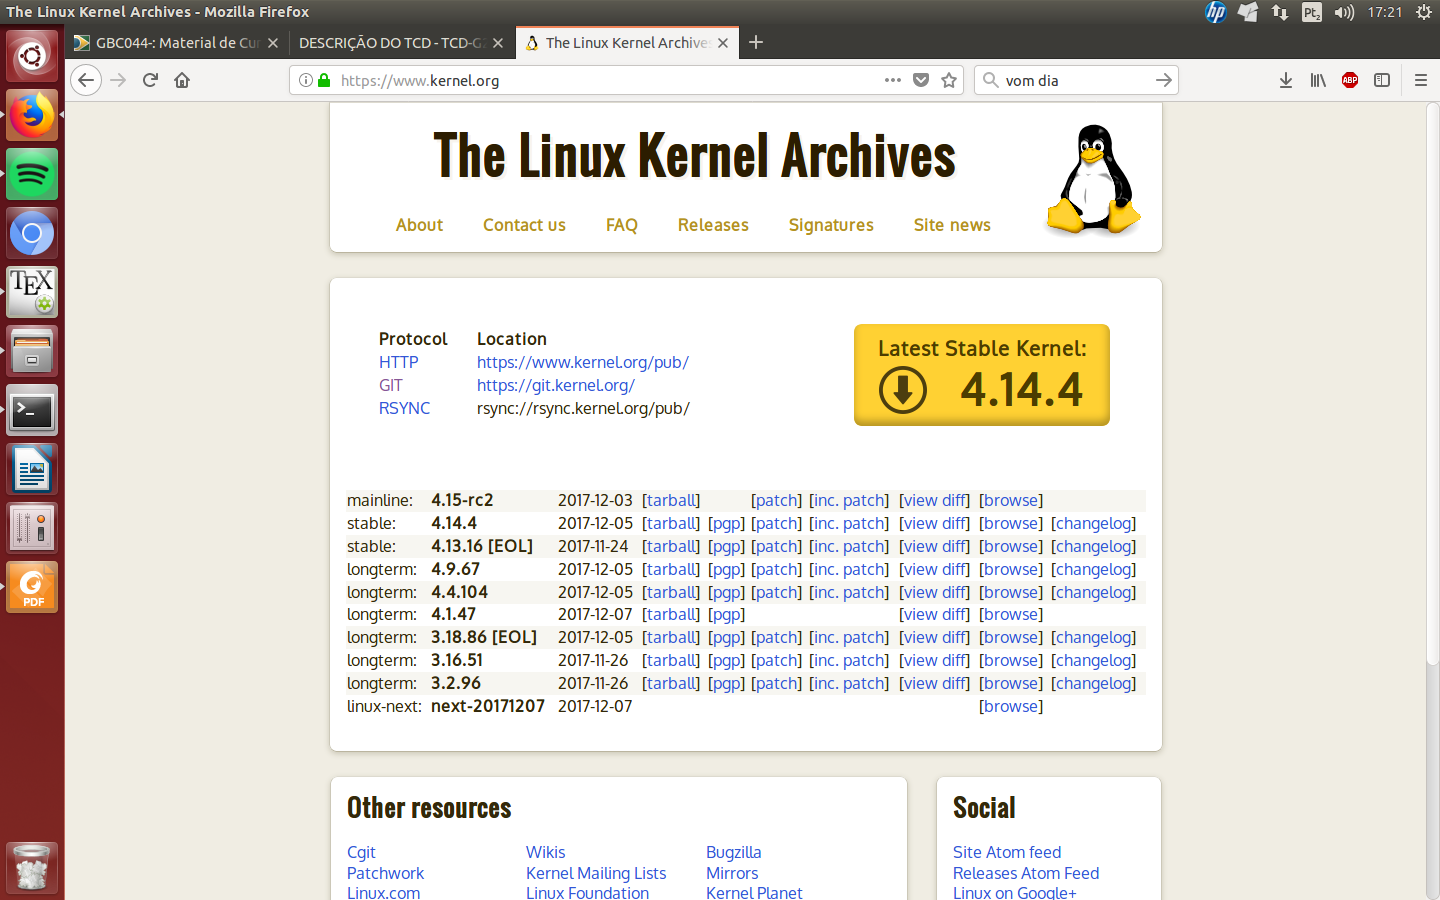
\includegraphics[scale=0.2]{imagens/kernelorg.png}
	\caption{The Linux Kernel Archives: Local de download do Kernel}
	\label{kernelorg}
\end{figure}
\subsection*{Compilação do kernel}
	Nesta seção vamos compilar o Kernel que previamente fizemos o Download para trabalhar com ele e assim poder cria nossas System Calls.
	Primeiramente precisamos instalar na nossa maquina um conjunto de ferramentas que nos permitira compilar nosso kernel, basta abrir seu terminal e digitar o seguinte comando:\newline
	\verb!sudo apt-­get install libncurses5­dev gcc make git exuberant­ctags! 
	Criamos uma pasta no nosso espaço de trabalho, posteriormente extraimos todo o conteudo do Kernel com o seguinte comando:\newline \verb!tar xvf linux­­*.tar.xz! \newline onde * é a versão do kernel que acabamos de fazer o download neste caso usamos linux-12.13.12, então ficou\newline
	\verb!tar xvf linux­3.17.1.tar.xz!\newline
	A seguir abrimos nossa pasta pelo terminal e acessamos onde está o kernel, fazendo uso do comando cd, que permite acessar um diretório.

	Agora vamos compilar nosso kernel completamente, para isso basta usar o comando make, porém existe algumas opções bem úteis para agilizar o processo para isso usamos: \newline
	\verb!make -­j4 CONFIG_LOCALVERSION="tutorial".! \newline
	Ao usar o -j4 estamos dizendo que o processo pode usar quandos processadores estejam disponiveis, no caso do exemplo saõ 4, ou seja, a maquina usada possui 4 processadores para realizar a tarefa, se sua maquina possuir 6, 8, etc você pode substituir pelo número de processadores da sua maquina,ou seja, jX, sendo x o número de processadores da sua maquina, vale resaltar que se precisa usar a máquina durante o processo é recomendavel deixar ao menos 1 processador para realizar suas atividas. Já o "tutorial" será o nome que seu kernel receberá após ser compilado e que você irá acessar quando estiver iniciando seu ubuntu, você pode alterar para o nome que desejar e fica entre "", pois, é um conjunto de caracteres, este processo pode demorar, pois, é um processo extremadamente grande, irá depender também da velocidade de processamento da máquina, em testes feitos pela nossas maquinas normalmente demorou entre 3 a 5 horas.
	\newline
	Quando por fim a compilação acabar precisamos substituir o kernel para assim que todas as modificações que fizermos posteriormente nele, possam ser carregadas com o sistema. Para isso abrimos o terminal vamos na pasta que criamos conforme a imagem anterior, e usamos os seguintes comandos: \newline
	\verb"make modules" \newline
	\verb"sudo make modules_install"\newline
	E por fim instalamos nosso novo kernel!, Este comando instala o Kernel, gera a imagem, copia os arquivos para o diretório /boot e atualiza o gerenciador de boot.\newline
	\verb"sudo make install" \newline;
	Agora está tudo pronto só precisamos acessar nosso novo kernel, para isso use no terminal o comando:\newline
	\verb"reboot" \newline
	
	Quando estiver na opção de escolher o Sistema Operacional basta acessar opções avançadas do ubuntu e selecionar o seu kernel, que estará identificado pelo nome inserido no começo, vale resaltar que quando você selecionar o kernel uma vez não é necessário selecionar-lo toda vez que der boot, a máquna pega o ultimo kernel instalado.
\subsection*{Criação da System Call}
A \textit{system call} foi criada dentro na pasta kernel no diretório principal deixando o arquivo  scall.c nessa pasta. Após isso foi adicionado o arquivo objeto no arquivo de \textit{makefile} como descrito no tutorial, dessa forma, foi encontrada no arquivo \textit{syscall\_64.tbl} na forma: \newline

\textbf{333	common	scall			sys\_det}
\newline
Assim a função pode ser chamada pela função \textit{\textbf{syscall(333)}} presente na \textit{unistd.h}. Por fim, foi adicionado o cabeçalho da função no arquivo \textit{syscall.h}. Depois disso foi compilado o kernel seguindo o tutorial proposto  %\cite{tutorial}. 
\\ \newline
\scriptsize{\textbf{unsigned long copy\_to\_user(void \_user *to, const void *from, unsigned long n)};}
\newline
	
Vejamos agora o código do kernel utilizado para

\subsubsection*{Tempo na CPU}
Como primeira tentativa para obter o tempo de CPU de um processo, acessamos a variável \textit{sum\_exec\_runtime} na estrutura \textit{task\_cputime}, com base nos comentários da estrutura, concluímos que tal variável era o que desejávamos como segue na figura 2: %fazer um hiperlink

\begin{figure}[!h]
	\centering
	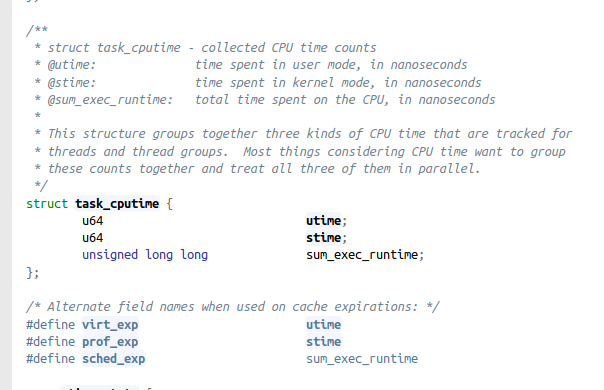
\includegraphics[scale=0.5]{imagens/img1.png}
	\caption{Estrutura task\_cputime}
	\label{taskcputime}
\end{figure}
	No entanto, com a tentativa não obtivemos o resultado esperado.
como segunda tentativa, encontramos uma função chamada get\_sum\_exec\_runtime

\begin{figure}[!h]
	\centering
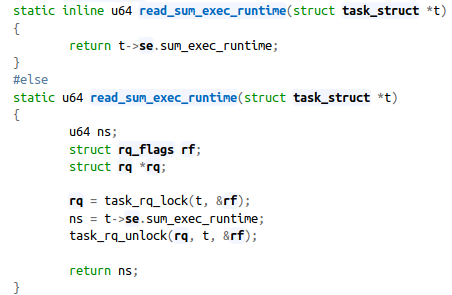
\includegraphics[scale=0.5]{imagens/sum_e.png} 
	\caption{sum\_exec\_runtime}
	\label{decschedentity}
\end{figure}

 Apartir de ai decidimos usar o que a função fornece, ou seja, chamar direto na propia task o desejado usando esse "su" que posteriormente seria a shed\_entity como segue a imagem:
 
\begin{figure}[!h]
	\centering
	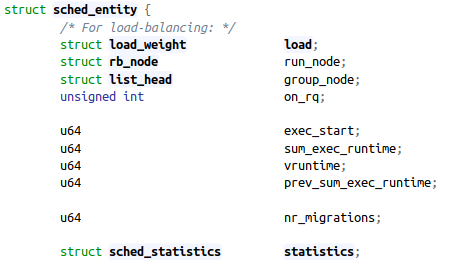
\includegraphics[scale=0.4]{imagens/img2.png}
	\caption{Parte da estrutura sched\_entity}
	\label{schedentity}
\end{figure}

	Que é o resultado que procuravamos, decidimos usar direto pois chamar uma função pode ser menos eficiente que chama-la na propia task\_struct assim obtemos em nano-segundos o tempo que o processo passou pela CPU.


\subsubsection*{Tempo de vida do processo}
\subsubsection*{N$^{\circ}$  de vezes que o processo passou pela CPU}
\subsection*{Código da system call}

\begin{figure}[!h]
	\centering
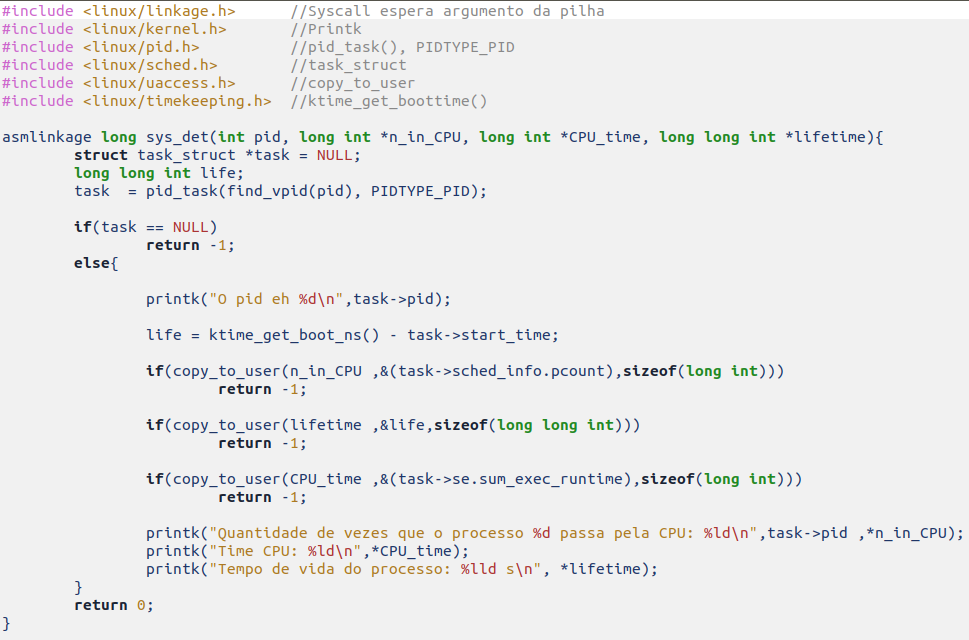
\includegraphics[scale=0.5]{imagens/codigosys.png} 
	\caption{Parte da estrutura sched\_entity}
	\label{codigosystem}
\end{figure}

Foi usada também a função copy\_to\_user para copiar um bloco de dados do kernel para o espaço de usuário para que a função possa retornar por parâmetro.

\subsection*{Programa usuário da system call}




\bibliographystyle{abbrv}
\bibliography{refs}
\end{document}
